\documentclass[11pt, oneside]{article}   	% use "amsart" instead of "article" for AMSLaTeX format
\usepackage[utf8]{inputenc}

\usepackage{lmodern}
\usepackage[T2A]{fontenc}
\usepackage{cmbright}
\usepackage[russian]{babel}
%\usetheme{Darmstadt}


\usepackage{amsmath}
\usepackage{amsfonts}
\usepackage{amssymb}
\usepackage{bm}
\usepackage{graphicx}
% Использовать полужирное начертание для векторов
\let\vec=\mathbf

\DeclareMathOperator{\mathspan}{span}
\DeclareMathOperator{\mathdim}{dim}
\DeclareMathOperator{\rank}{rank}
\DeclareMathOperator{\diag}{diag}
\begin{document}
	\author{Е. Ларин, Ф. Ежов, И. Кононыхин }
	\title{Neural Nets (NN), с элементами Deep Learning}
	\date{}
	
	\maketitle
	\section{Математическая модель нейрона}
	
	Биологический нейрон состоит из тела диаметром от 3 до 100 мкм, содержащего ядро, другие органеллы и отростки. Выделяют два вида отростков. Аксон — обычно длинный отросток, приспособленный для проведения возбуждения от тела нейрона. Дендриты — как правило, короткие и сильно разветвлённые отростки, служащие главным местом образования влияющих на нейрон возбуждающих и тормозных синапсов (разные нейроны имеют различное соотношение длины аксона и дендритов). Нейрон может иметь несколько дендритов и обычно только один аксон. Один нейрон может иметь связи с 20 тысячами других нейронов. Кора головного мозга человека содержит около 80 миллиардов нейронов. 
	
	\begin{figure}[h]
		\center{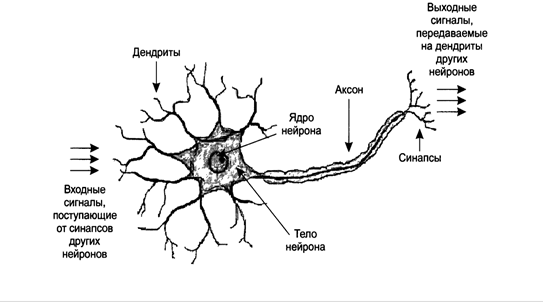
\includegraphics[width=1\linewidth]{../Report/imgs/bio_neuron}}
	\end{figure}


	\subsection{Перцептрон (Перцептрон Розенблатта)}	
	
	Математическая модель искусственного нейрона была предложена У. Маккалоком и У. Питтсом вместе с моделью сети, состоящей из этих нейронов. Авторы показали, что сеть на таких элементах может выполнять числовые и логические операции. Практически сеть была реализована Фрэнком Розенблаттом в 1958 году как компьютерная программа, а впоследствии как электронное устройство — перцептрон. Первоначально нейрон мог оперировать только с сигналами логического нуля и логической единицы, поскольку был построен на основе биологического прототипа, который может пребывать только в двух состояниях — возбужденном или невозбужденном. Развитие нейронных сетей показало, что для расширения области их применения необходимо, чтобы нейрон мог работать не только с бинарными, но и с непрерывными (аналоговыми) сигналами. Такое обобщение модели нейрона было сделано Уидроу и Хоффом, которые предложили в качестве функции срабатывания нейрона использовать логистическую кривую.
	
	Связи, по которым выходные сигналы одних нейронов поступают на входы других, часто называют синапсами по аналогии со связями между биологическими нейронами. Каждая связь характеризуется своим весом. Связи с положительным весом называются возбуждающими, а с отрицательным — тормозящими. Нейрон имеет один выход, часто называемый аксоном по аналогии с биологическим прототипом. С единственного выхода нейрона сигнал может поступать на произвольное число входов других нейронов.
	
	Математически нейрон представляет собой взвешенный сумматор, единственный выход которого определяется через его входы и матрицу весов.
	
	Введем обозначения:
	
	\begin{itemize}
		\item $p$ --- количество признаков
		\item $\{ x_1, \cdots, x_p \}$ --- индивид (сигналы на входах нейрона). 
		\item $\{ w_1, \cdots, w_p \}$ --- веса нейрона. 
		\item Функция активации \begin{equation*} 
			f(h) =  \begin{cases}
				0 & h < 0 \\
				1 & h \geqslant 0
			\end{cases}
		\end{equation*}
		\item $y$ --- выход сети.
	\end{itemize}

	\begin{figure}[h]
		\centering
		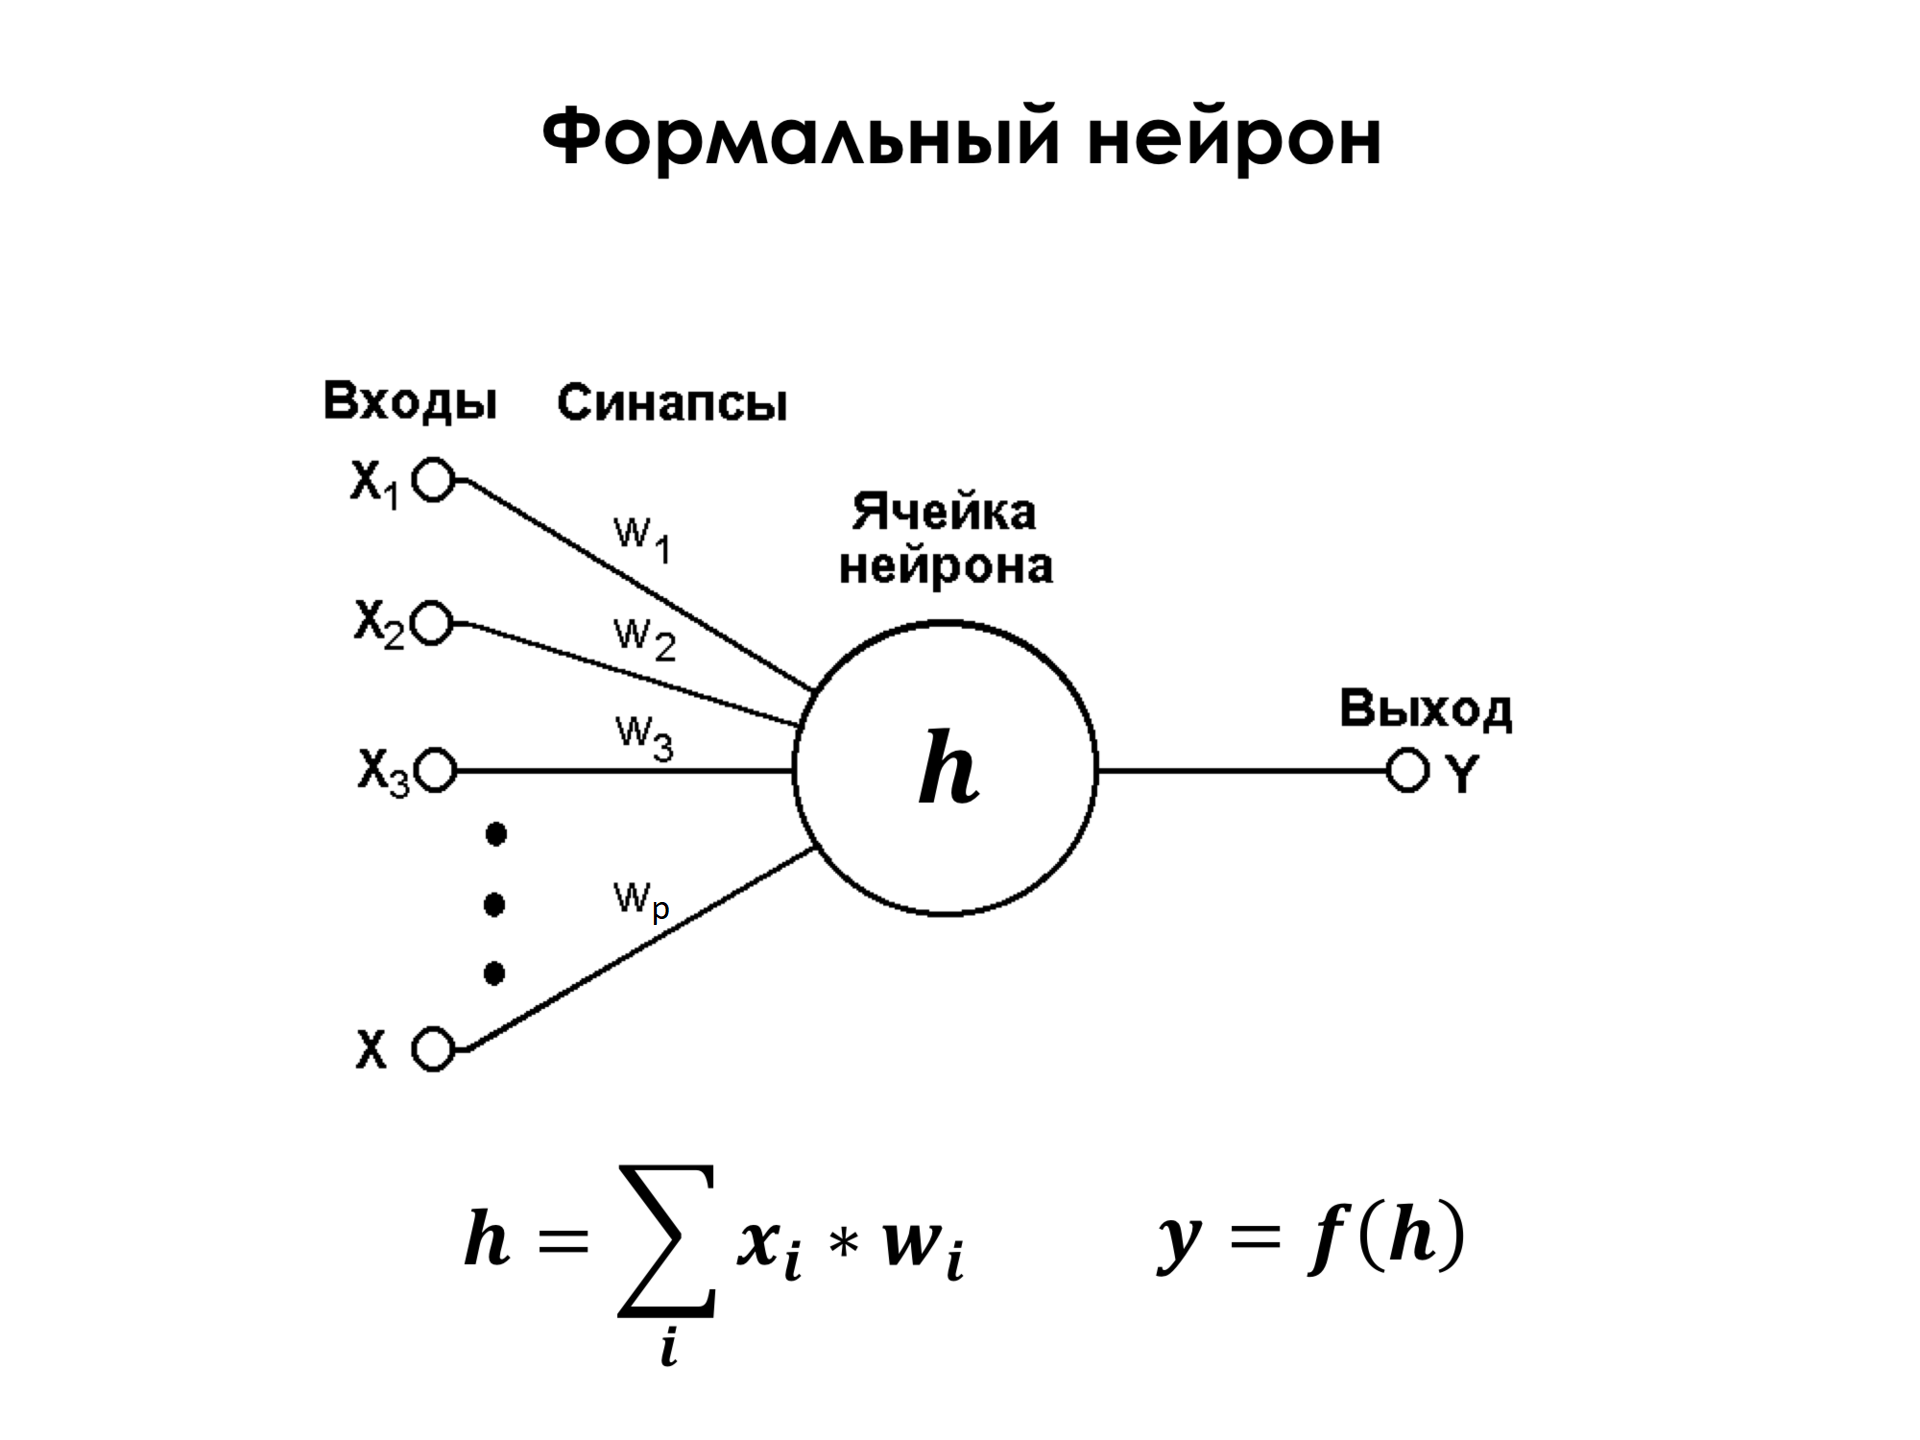
\includegraphics[width=0.7\linewidth]{imgs/math_neuron}
	\end{figure}
	
	Тогда формально математическую модель перцептрона можно определить как:
	$$ y = f(h) = f(\sum\limits_{i=1}^{p} x_i w_i + x_0w_0) $$.
	Возможные значения сигналов на входах нейрона считают заданными в интервале $ [0,1] $.
	Дополнительный вход $ x_{0} $ и соответствующий ему вес $ w_{0} $ используются для инициализации нейрона. Под инициализацией подразумевается смещение активационной функции нейрона по горизонтальной оси, то есть формирование порога чувствительности нейрона. Кроме того, иногда к выходу нейрона специально добавляют некую случайную величину, называемую сдвигом. Сдвиг можно рассматривать как сигнал на дополнительном, всегда нагруженном, синапсе.

	К сожалению, перцептрон может решать только линейно разделимые задачи. Он не способен решить некоторые тривиальные задачи, например задачу классификации на основе исключающего "ИЛИ" (Exclusive OR - XOR). 
	
	\subsection{Многослойный перцептрон (Многослойный перцептрон Румельхарта)}
	
	В многослойном перцептроне каждый слой кроме выходного включает нейрон смещения и полностью связан со следующим слоем.\\
	
	\begin{figure}[h]
		\center{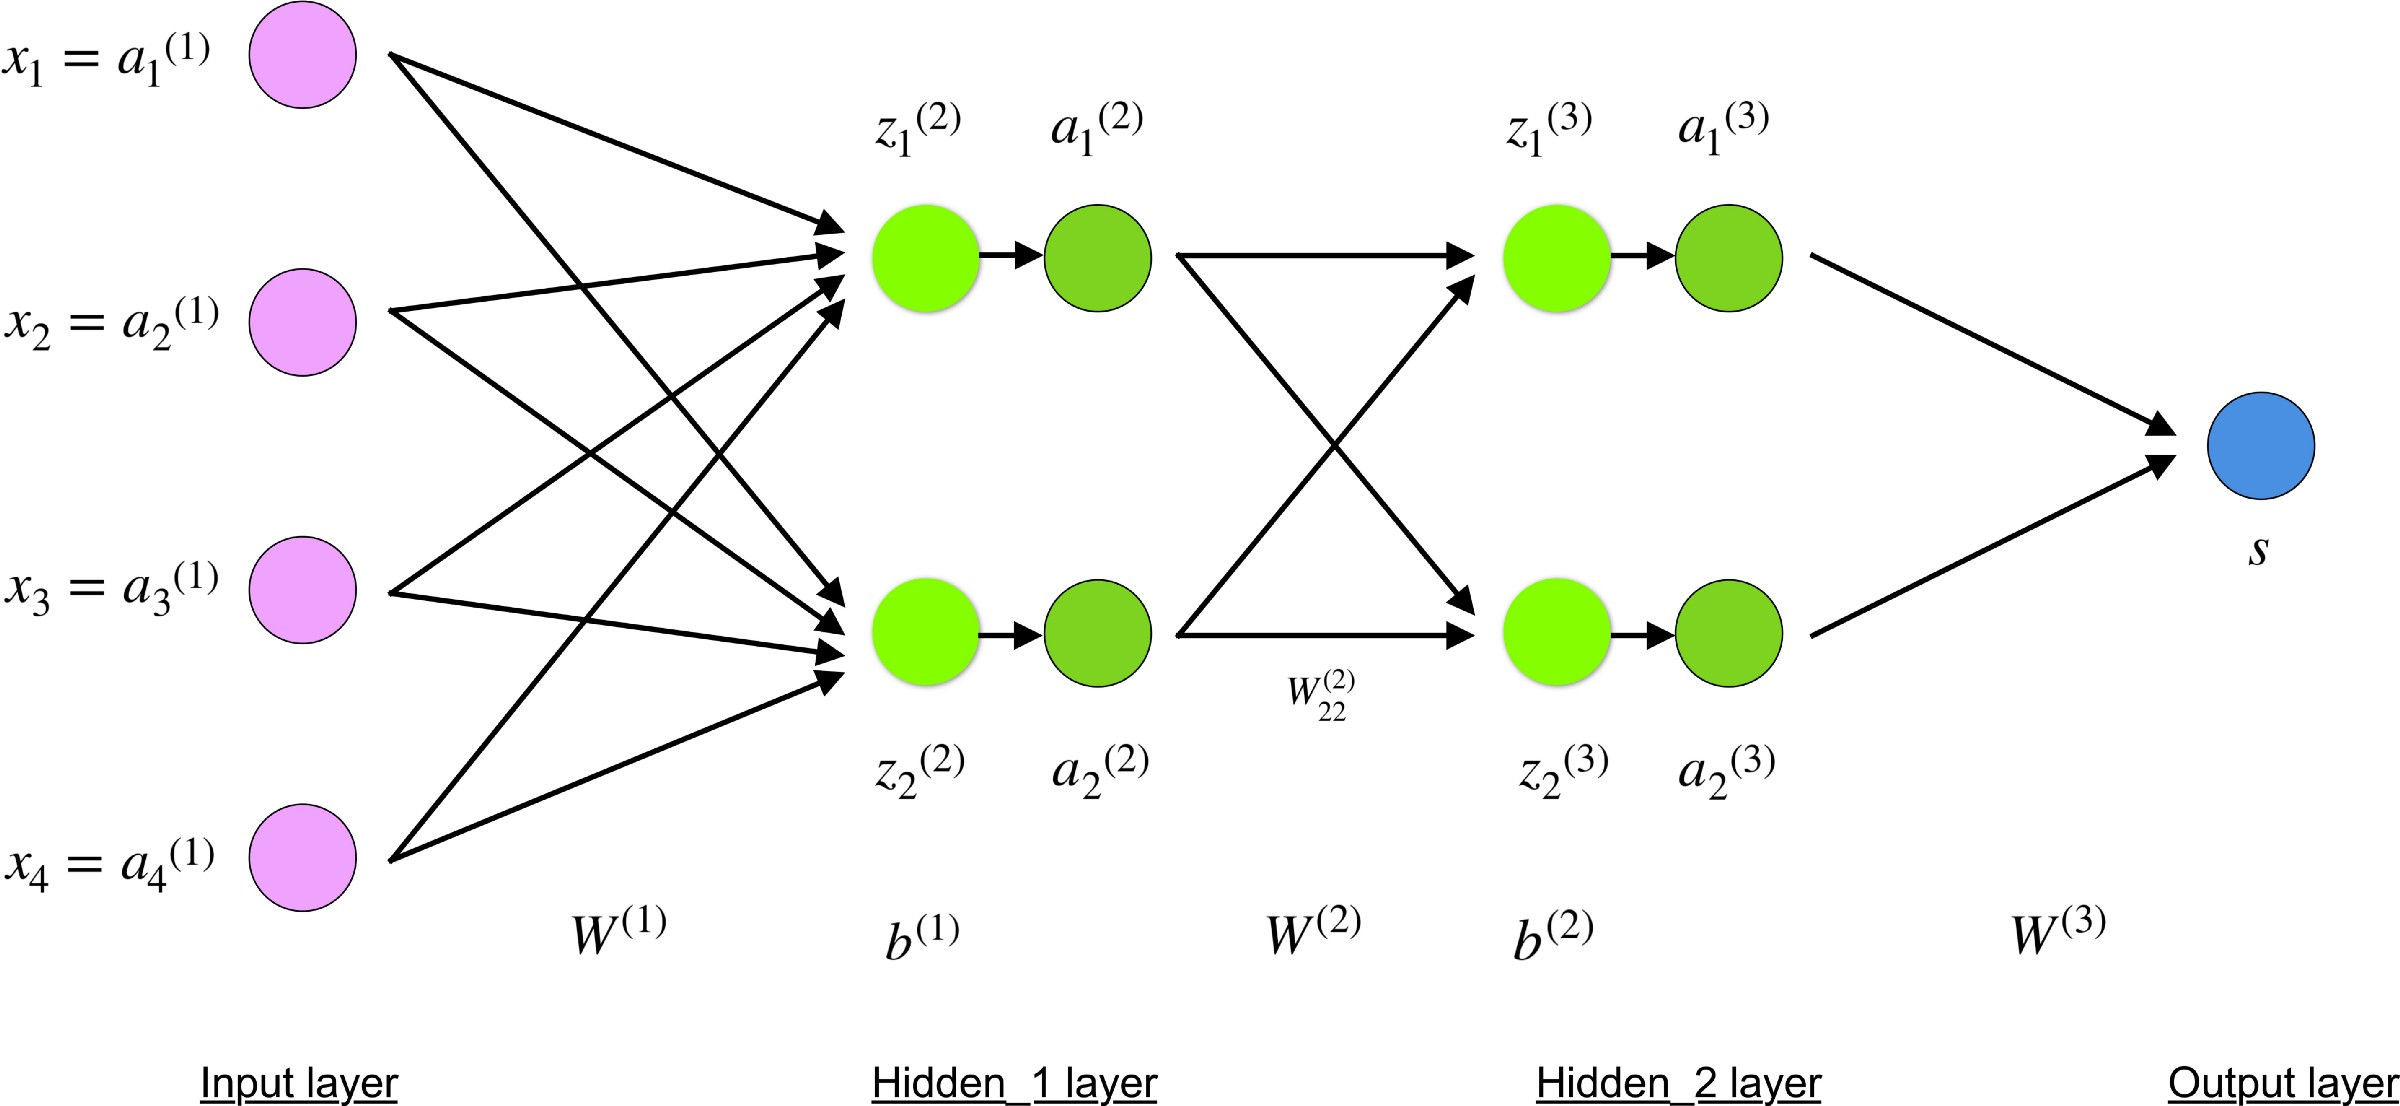
\includegraphics[width=1\linewidth]{../Report/imgs/MLP}}
	\end{figure}
	Обозначим функцию $\sigma(z)$ --- сигмоидой, если $\lim\limits_{z 	\rightarrow -\infty}\sigma(z) = 0$ и $\lim\limits_{z 	\rightarrow +\infty}\sigma(z) = 1$.
	
	
	\textbf{Теорема Цыбенко}: \\
		Если функция активации $\sigma(z)$ --- непрерывная сигмоида, то для любой непрерывной на $[0, 1]^p$ функции $f(x)$ существуют такие значение параметров $w_h \in \mathbb{R}^p, w_0 \in \mathbb{R}, \alpha_h \in \mathbb{R} $, что двухслойная сеть 
		$$ a(x) = \sum\limits_{h=1}^H \alpha_h \sigma( \langle x, w_h \rangle + w_0) $$
		
		равномерно приближает $f(x)$ с любой точность $\varepsilon$:
		$$ |a(x) - f(x)| < \varepsilon, \text{для всех } x \in [0, 1]^p $$
	
	Данная теорема говорит о том, что с помощью линейных операций и одной нелинейной функции активации можно приблизить любую непрерывную функцию с любой желаемой точностью.\\
	
	\newpage
	Функции активации:
	\begin{figure}[h]
		\center{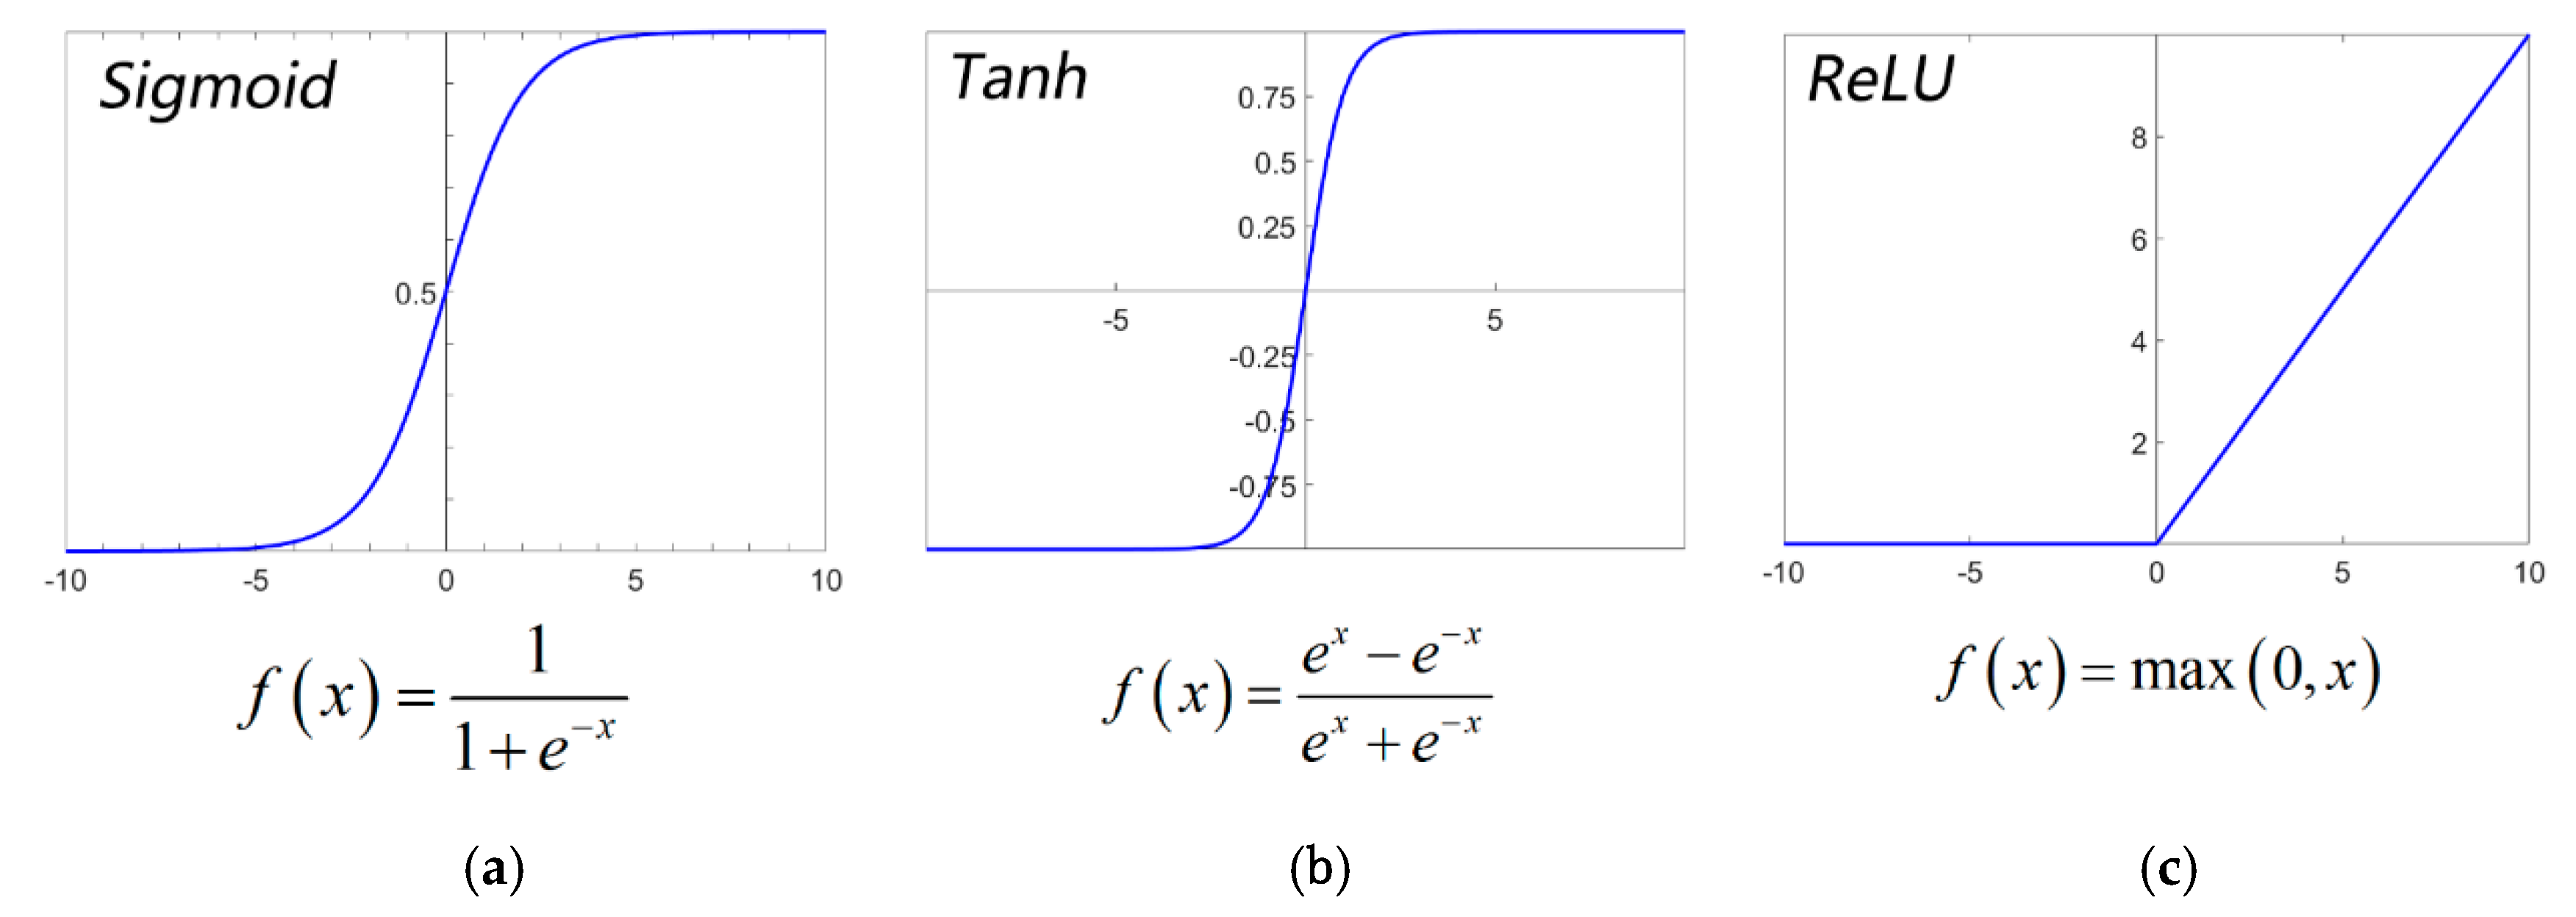
\includegraphics[width=1\linewidth]{../Report/imgs/afuns}}
	\end{figure}
	
	\section{Обучение MLP}
	Задачей оптимизации является минимизация средних потерь на обучающей выборке:
	$$ Q(w) := \dfrac{1}{n} \sum\limits_{i=1}^{n} \mathcal{C}_i(w) \rightarrow \min\limits_w  $$
	$\mathcal{C}$ --- любая дифференцируемая функция потерь. \\
	
	\textbf{Обучение методом стохастического градиента.}
	
	Вход: выборка $X^n$; <<скорость>> обучение $\epsilon$; параметр $\lambda$;
	
	Выход: оптимизированные значение весов $w$.
	
	\begin{enumerate}
		\item инициализация весов $w$ и текущую оценку $Q(w)$
		\item повторять
		\item выбрать объект $x_i$ из $X^n$;
		\item вычислить потерю $\mathcal{C}_i := \mathcal{C}_i(w)$
		\item градиентный шаг: $w := w - \epsilon \mathcal{C}_i^{'}(w)$
		\item оценить значение функционала: $Q := (1-\lambda)Q + \lambda \mathcal{C}_i$
		\item пока значение $Q$ и/или весов $w$ не стабилизируются
	\end{enumerate}	

	\newpage
	Обучение MLP разделяют на 2 этапа - forward и backward propogation.
	Forward propogation относится к подсчету функционала $ Q $ на текущей итерации, в то время как backward prop - к обновлению весов сети.
	
	\begin{figure}[h]
		\center{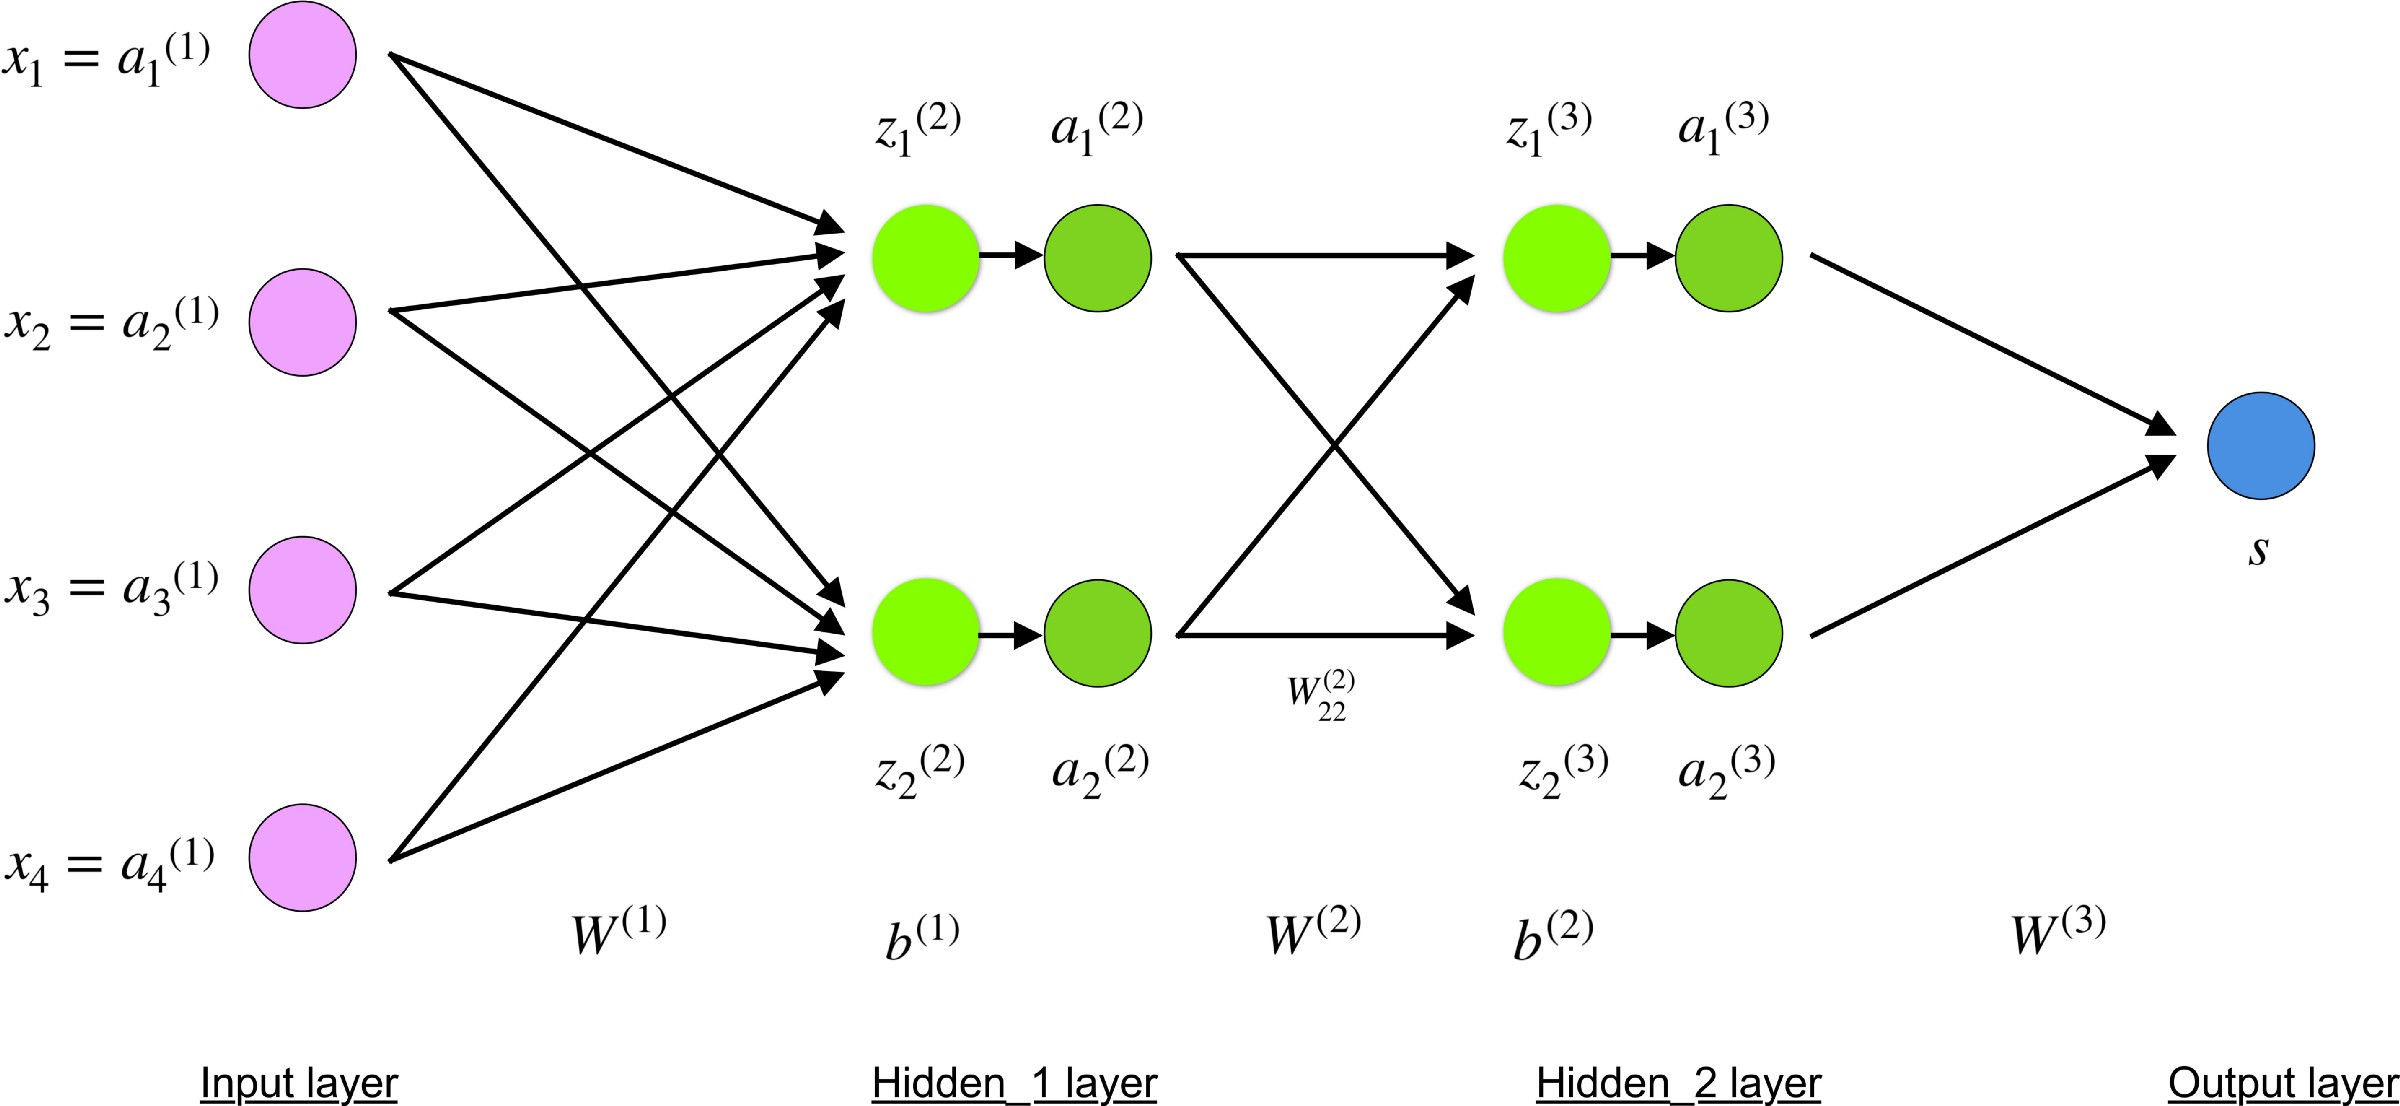
\includegraphics[width=1\linewidth]{../Report/imgs/MLP}}
	\end{figure}
	
	Forward prop.
	\begin{figure}[h]
		\center{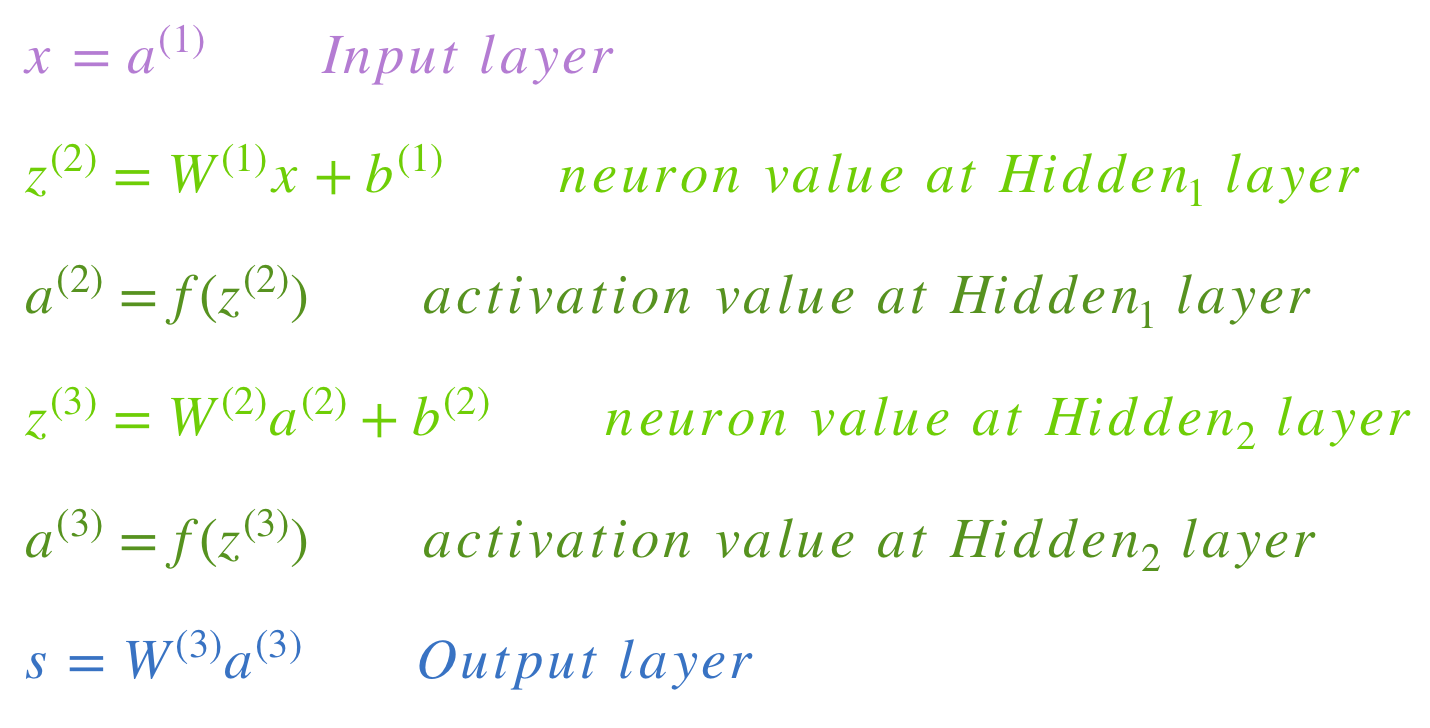
\includegraphics[width=0.6\linewidth]{../Report/imgs/forwardprop}}
	\end{figure}
	
	\begin{figure}[h]
		\center{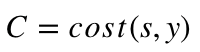
\includegraphics[width=0.2\linewidth]{../Report/imgs/cost_function}}
	\end{figure}
	
	$s$ --- полученная оценка с помощью нейронной сети. $y$ --- правильный ответ. $\mathcal{C}$ --- значение ошибки между $s$ и $y$ по какой-нибудь метрики (например MSE).
	
	\newpage
	Backward prop.
	\begin{figure}[h]
		\center{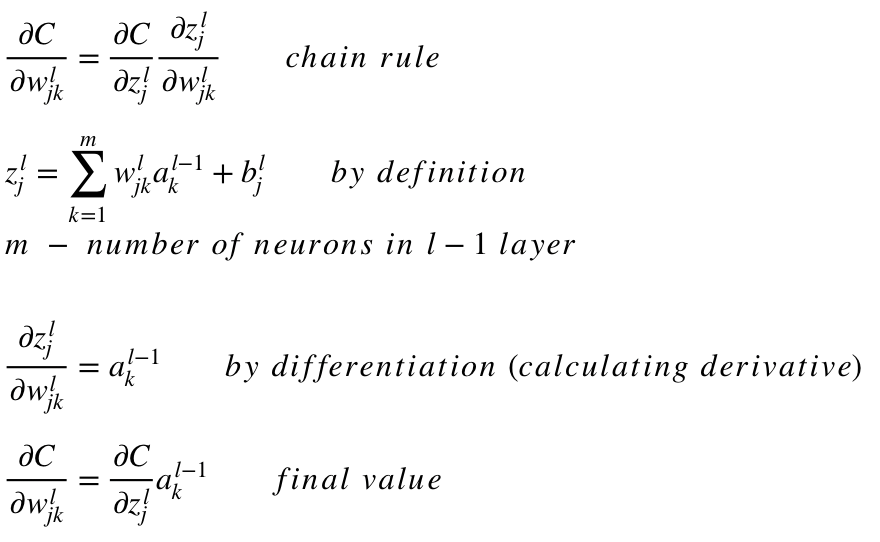
\includegraphics[width=0.7\linewidth]{../Report/imgs/chain-rule}}
	\end{figure}

	Отсюда, изменение весов сети выглядит следующим образом:
	
	\begin{figure}[h]
		\center{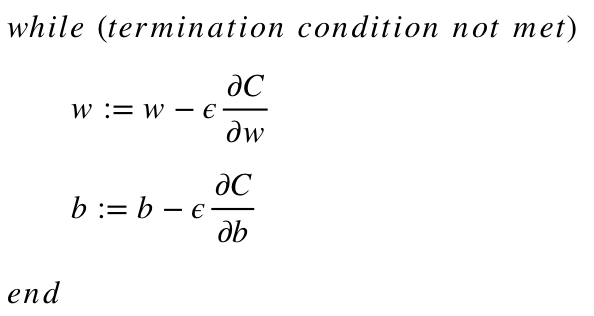
\includegraphics[width=0.7\linewidth]{../Report/imgs/weigh_change_process}}
	\end{figure}
	
	
	Преимущества:
	\begin{itemize}
		\item быстрое вычисление градиента
		\item обобщение на любые функции активации, функции потерь и количество слоев
		\item возможность потокового обучения
		\item возможность распараллеливания
	\end{itemize}
	
	Недостатки: 
	\begin{itemize}
		\item медленная сходимость
		\item застревания в локальных экстремумах
		\item проблема переобучения
	\end{itemize}
	
	На сегодняшний день алгоритм стохастического градиента считается устаревшим и редко используется для обучения нейронных сетей. Более быстрыми модификациями являются:
	\begin{itemize}
		\item Stochastic Gradient (SG)
		\item Метод накопления импульса (Momentum)
		\item NAG (Nesterov's accelerated gradient)
		\item RMSProp (running mean square)
		\item AdaDelta (adaptive learning rate)
		\item Adam (adaptive momentum)
		\item Nadam (Nesterov-accelerated adaptive momentume)
	\end{itemize}
	
	\newpage
	\section{Recurrent neural network(RNN)}
	Рекуррентные нейронные сети — вид нейронных сетей, где связи между элементами образуют направленную последовательность. Благодаря этому появляется возможность обрабатывать серии событий во времени или последовательные пространственные цепочки. В отличие от многослойных перцептронов, рекуррентные сети могут использовать свою внутреннюю память для обработки последовательностей произвольной длины. Поэтому сети RNN применимы в таких задачах, где нечто целостное разбито на части, например: 
	\begin{itemize}
		\item Прогнозирование временных рядов
		\item Управление технологическими процессами
		\item Классификация текстов или их фрагментов
		\item Анализ тональности документа / предложений / слов
		\item Машинный перевод
		\item Распознавание речи
		\item Синтез речи
		\item Синтез ответов на вопросы, разговорный интеллект
		\item Генерация подписей к изображениям
		\item Генерация рукописного текста
		\item Интерпретация генома и другие задачи биоинформатики
	\end{itemize}
	
	\newpage
	Введем обозначения:\\
	$x_t$ --- входной вектор в момент времени $t$\\
	$s_t$ --- вектор скрытого слоя в момент времени $t$\\
	$y_t$ --- выходной вектор (в некоторых случаях $y_t \equiv s_t$)
	
	\begin{figure}[h]
		\center{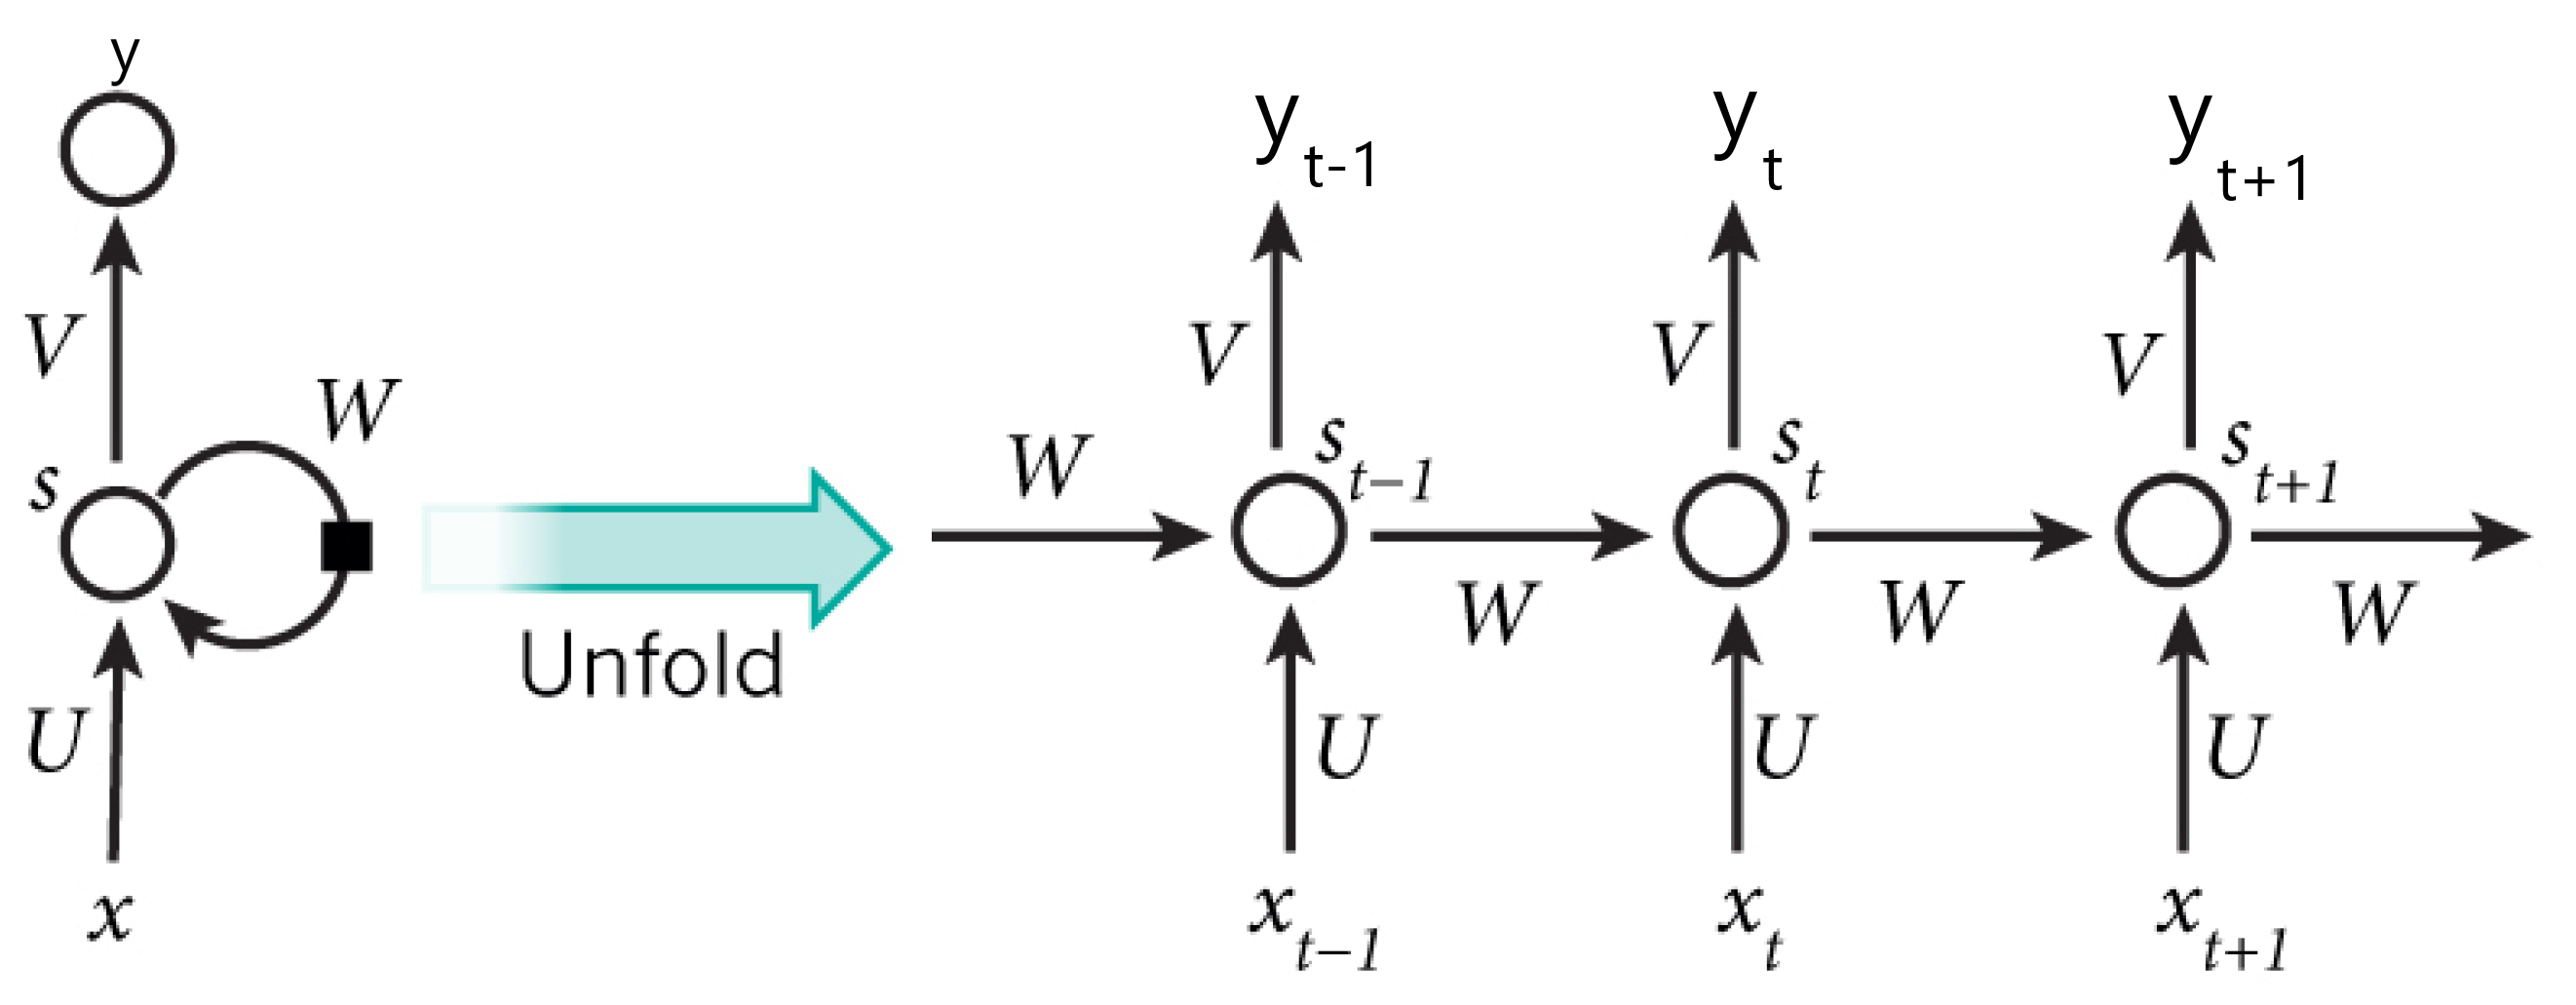
\includegraphics[width=0.8\linewidth]{../Report/imgs/rnn}}
	\end{figure}
	
	Задача:
	$$ \sum\limits_{t=0}^{T}\mathcal{C}_t(U, V, W) \rightarrow \min\limits_{U, V, W}$$
	
	$\mathcal{C}_t(U, V, W) = \mathcal{C}(y_t(U, V, W))$ --- потеря от предсказания $y_t$.
	
	Обучаются рекуррентные сети методом Back-propagation Through Time (BPTT).
	
	$$ \dfrac{\partial\mathcal{C}_t}{\partial W} = \dfrac{\partial\mathcal{C}_t}{\partial y_t} \dfrac{\partial y_t}{\partial s_t} \sum\limits_{k=0}^{t} \bigg(  \prod\limits_{i = k+1}^{t}  \dfrac{\partial s_i}{\partial s_{i-1}} \bigg)  \dfrac{\partial h_k}{\partial W}$$
	
	\begin{figure}[h]
		\center{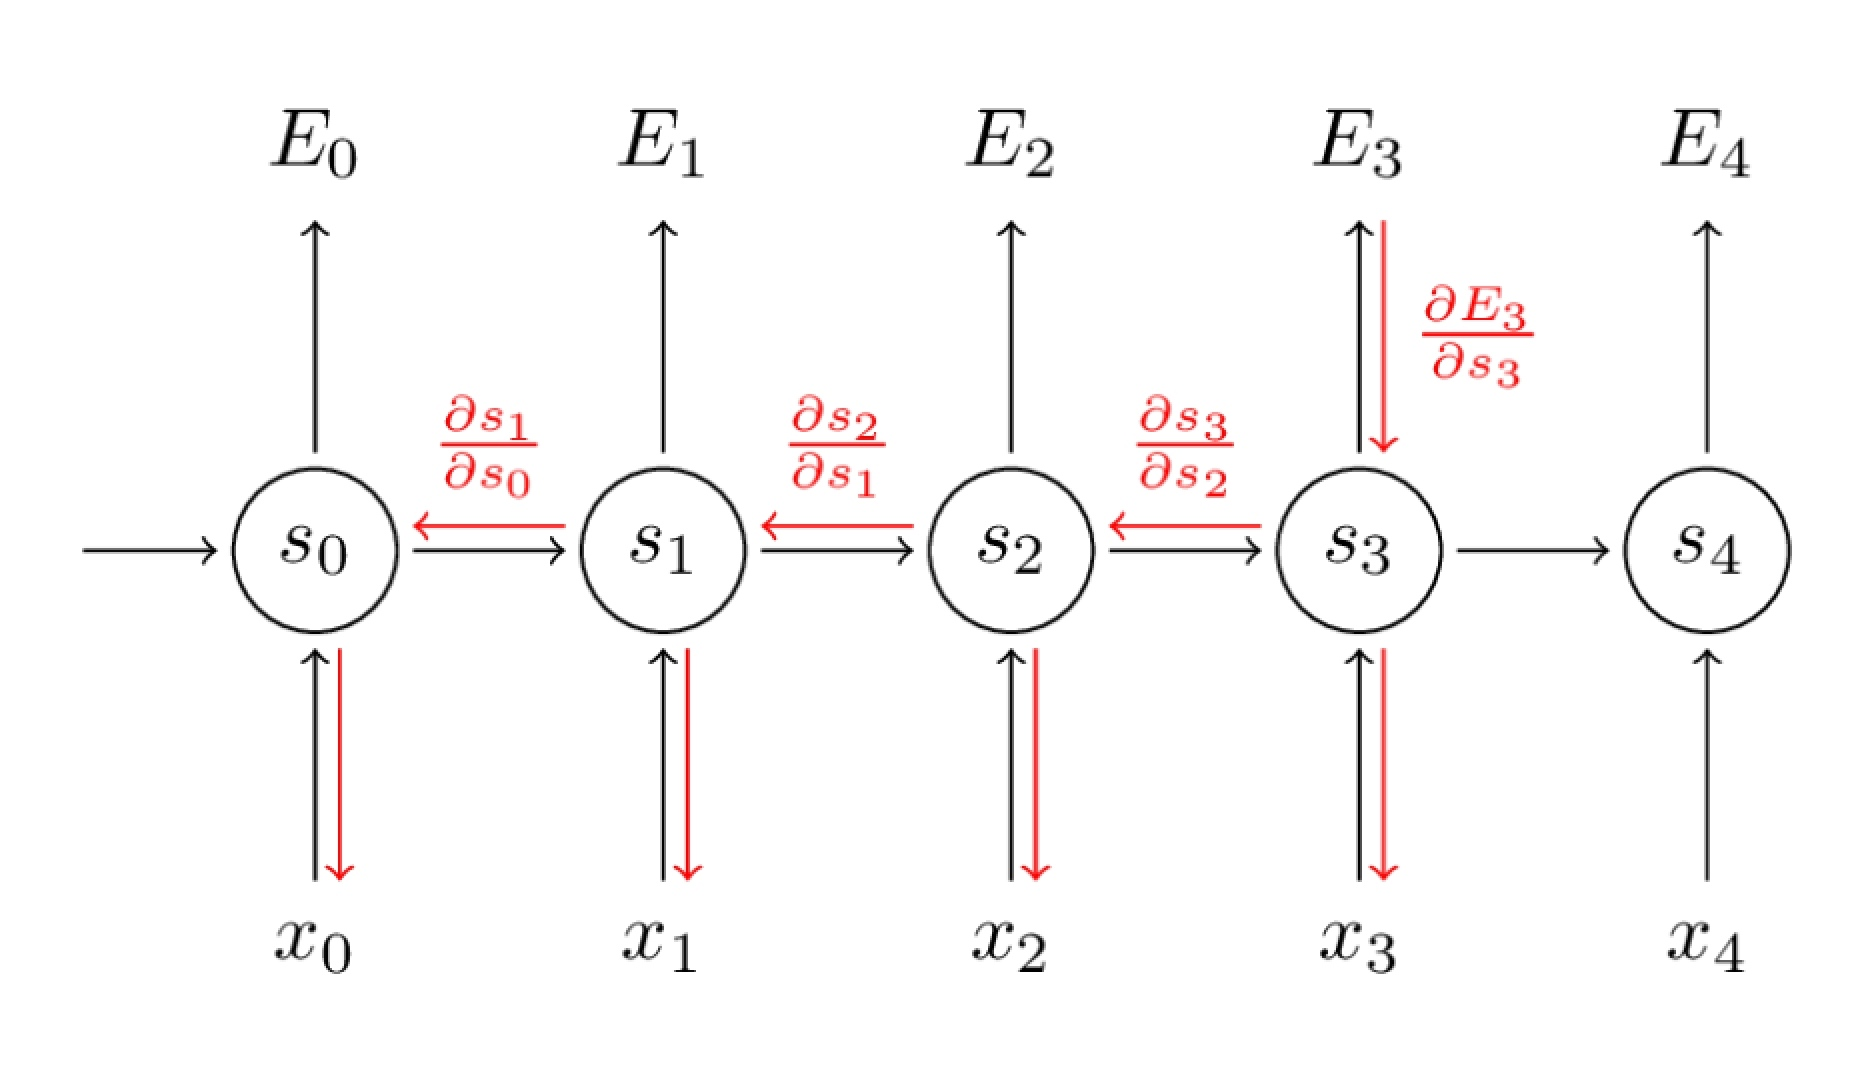
\includegraphics[width=0.8\linewidth]{../Report/imgs/bptt}}
	\end{figure}
	
	\newpage
	\section{LSTM}
	В отличие от традиционных рекуррентных нейронных сетей, LSTM-сеть хорошо приспособлена к обучению на задачах классификации, обработки и прогнозирования временных рядов в случаях, когда важные события разделены временными лагами с неопределённой продолжительностью и границами. Относительная невосприимчивость к длительности временных разрывов даёт LSTM преимущество по отношению к альтернативным рекуррентным нейронным сетям, скрытым марковским моделям и другим методам обучения для последовательностей в различных сферах применения.\\
	Мотивация LSTM: сеть должна долго помнить контекст, какой именно --- сеть должна выучить сама. Вводится $C_t$ --- вектор состояния сети в момент $t$.
	
	Архитектура: 
	\begin{figure}[h]
		\center{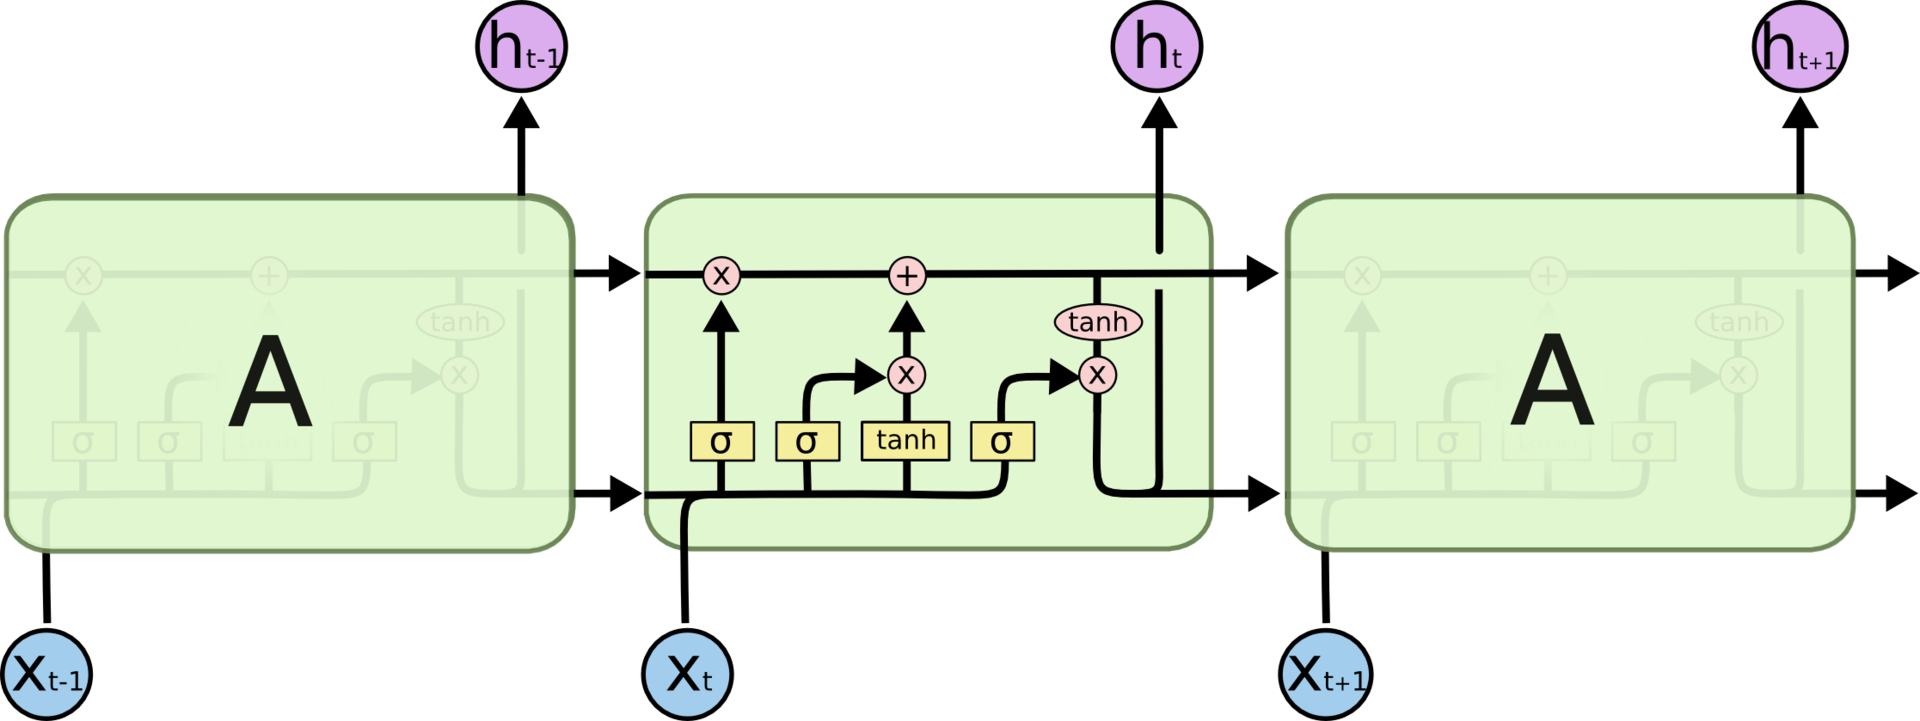
\includegraphics[width=1\linewidth]{../Report/imgs/lstm}}
	\end{figure}
	
	\begin{figure}[h]
		\center{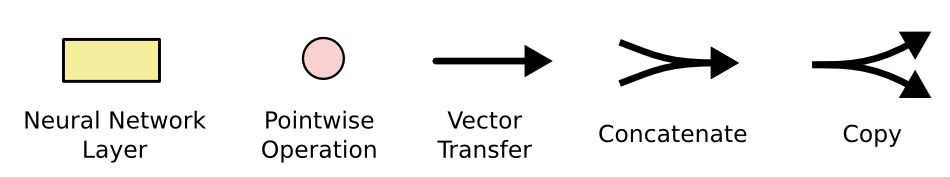
\includegraphics[width=0.8\linewidth]{../Report/imgs/lstm_operations}}
	\end{figure}
	
	\newpage
	Шаг 1:
	\begin{figure}[h]
		\center{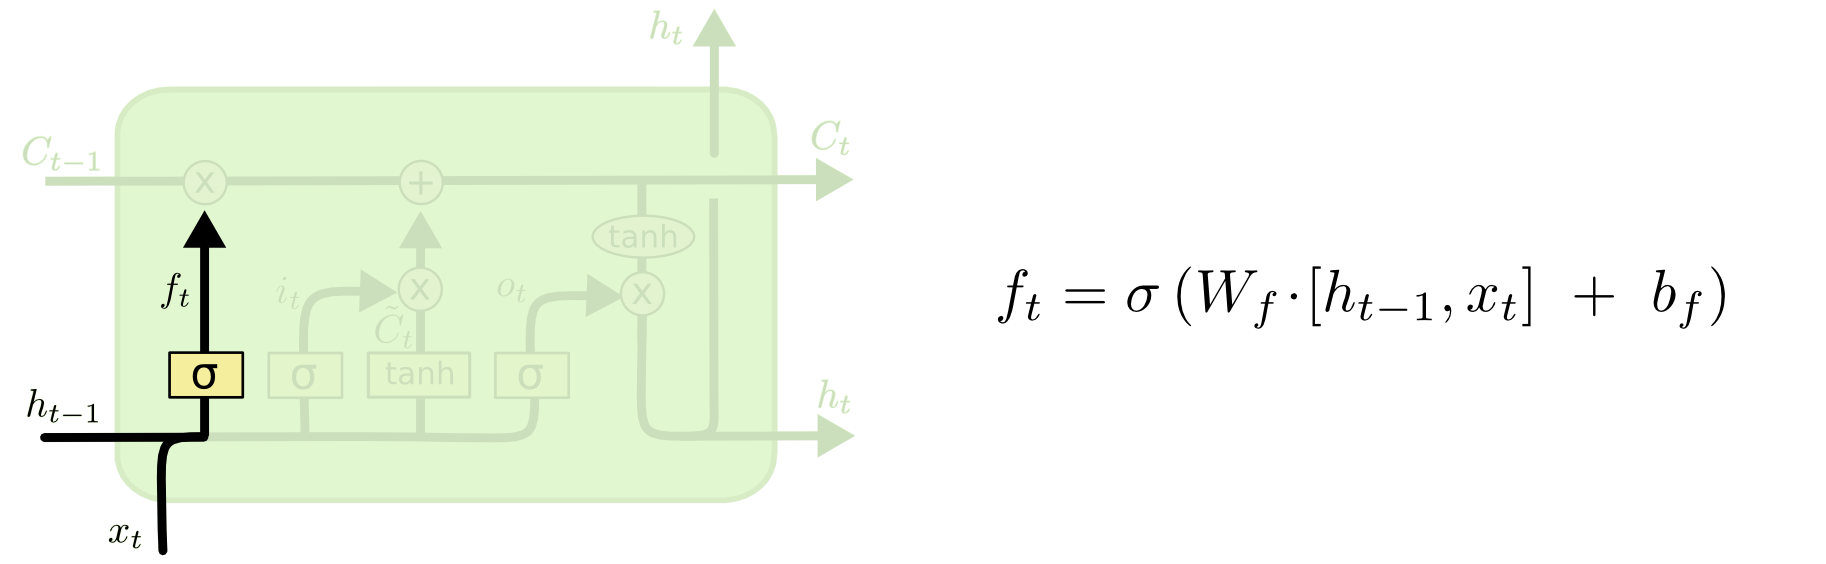
\includegraphics[width=1\linewidth]{../Report/imgs/lstm_explanation_step1}}
	\end{figure}

	Шаг 2:
	\begin{figure}[h]
		\center{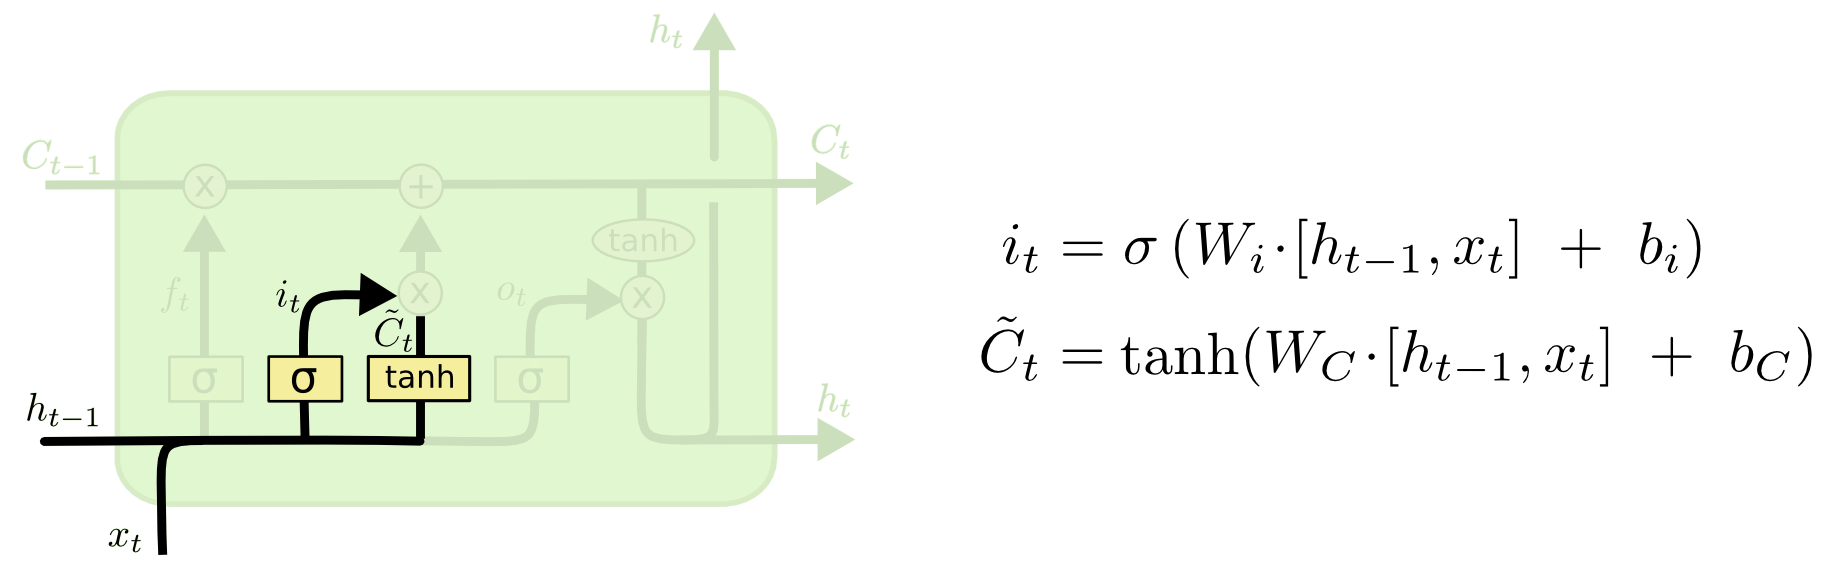
\includegraphics[width=1\linewidth]{../Report/imgs/lstm_explanation_step2}}
	\end{figure}
	
	
	Шаг 3:
	\begin{figure}[h]
		\center{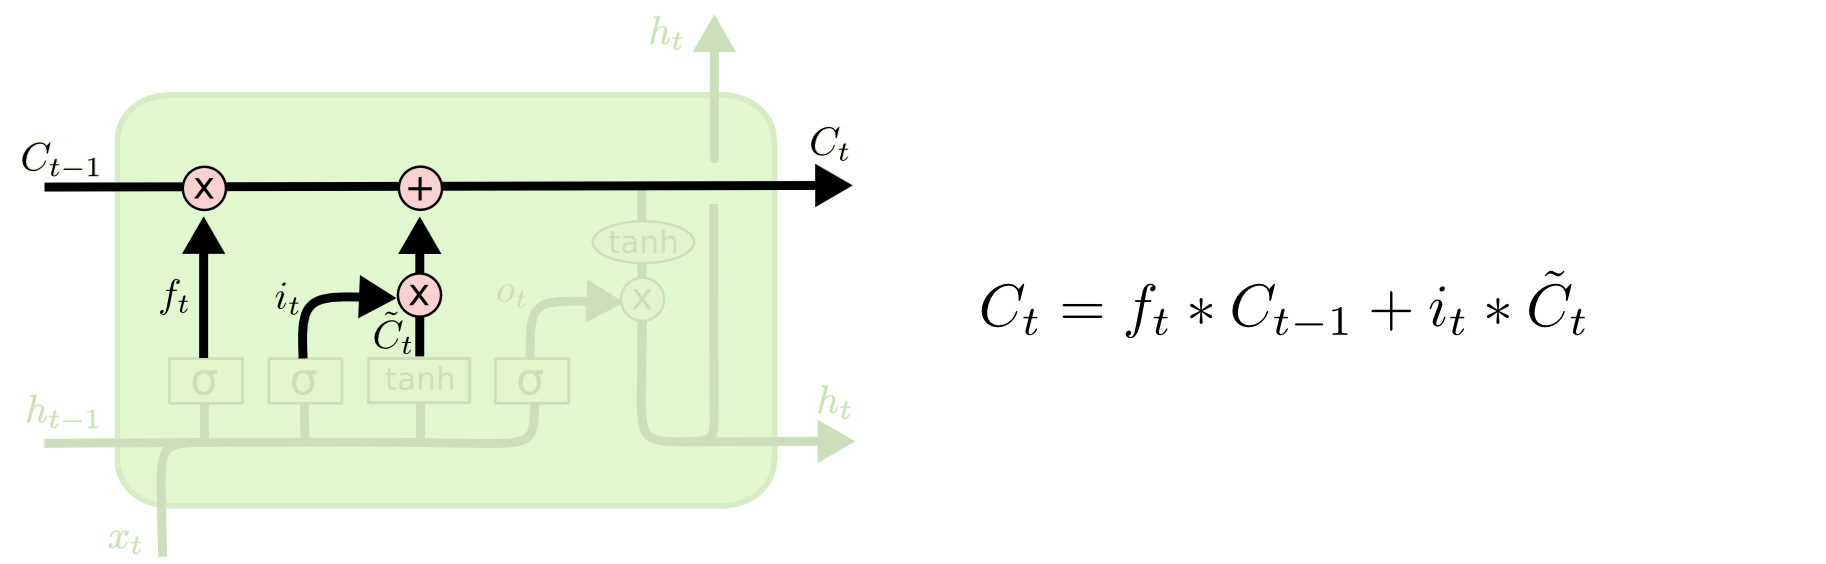
\includegraphics[width=1\linewidth]{../Report/imgs/lstm_explanation_step3}}
	\end{figure}
	
	\newpage
	Шаг 4:
	\begin{figure}[h]
		\center{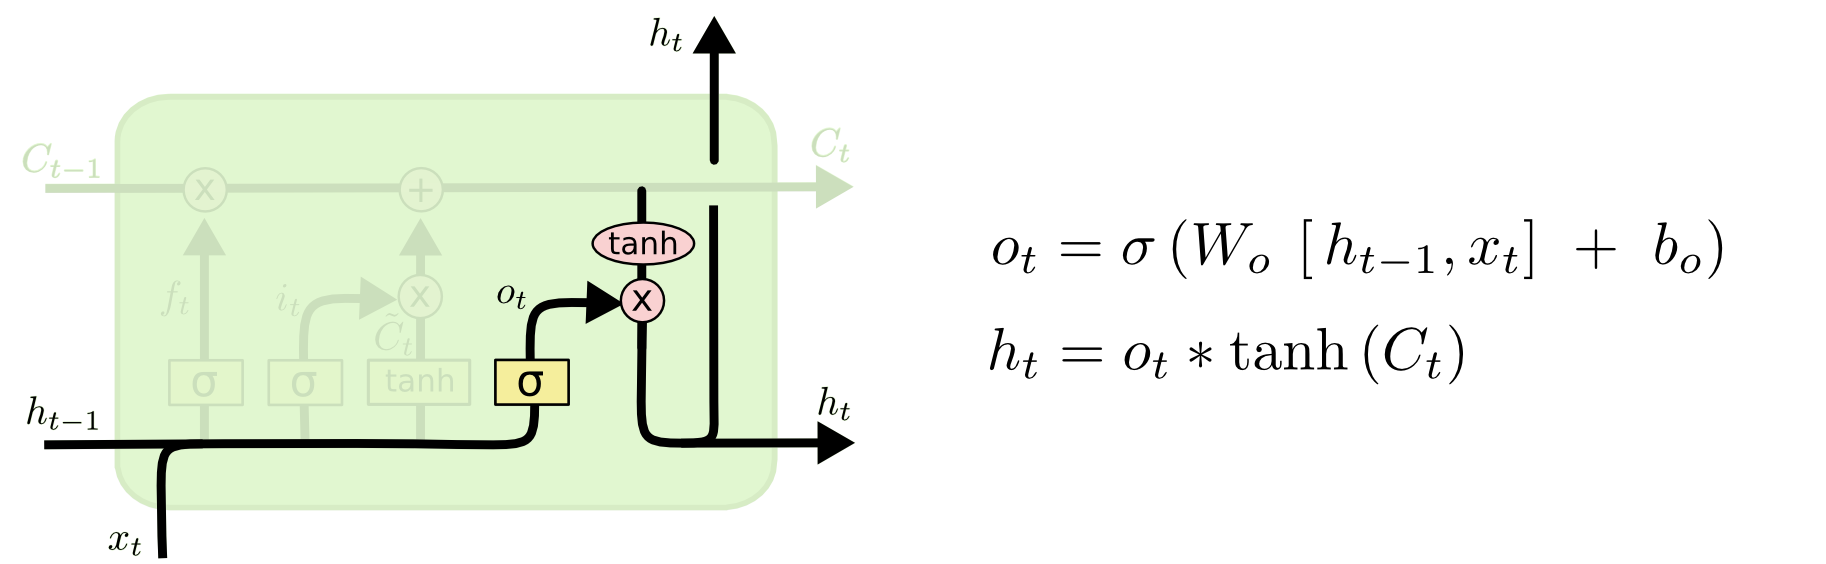
\includegraphics[width=1\linewidth]{../Report/imgs/lstm_explanation_step4}}
	\end{figure}
	
	
	\textbf{LSTM с <<замочными скважинами>> (peepholes)}
	
	\begin{figure}[h]
		\center{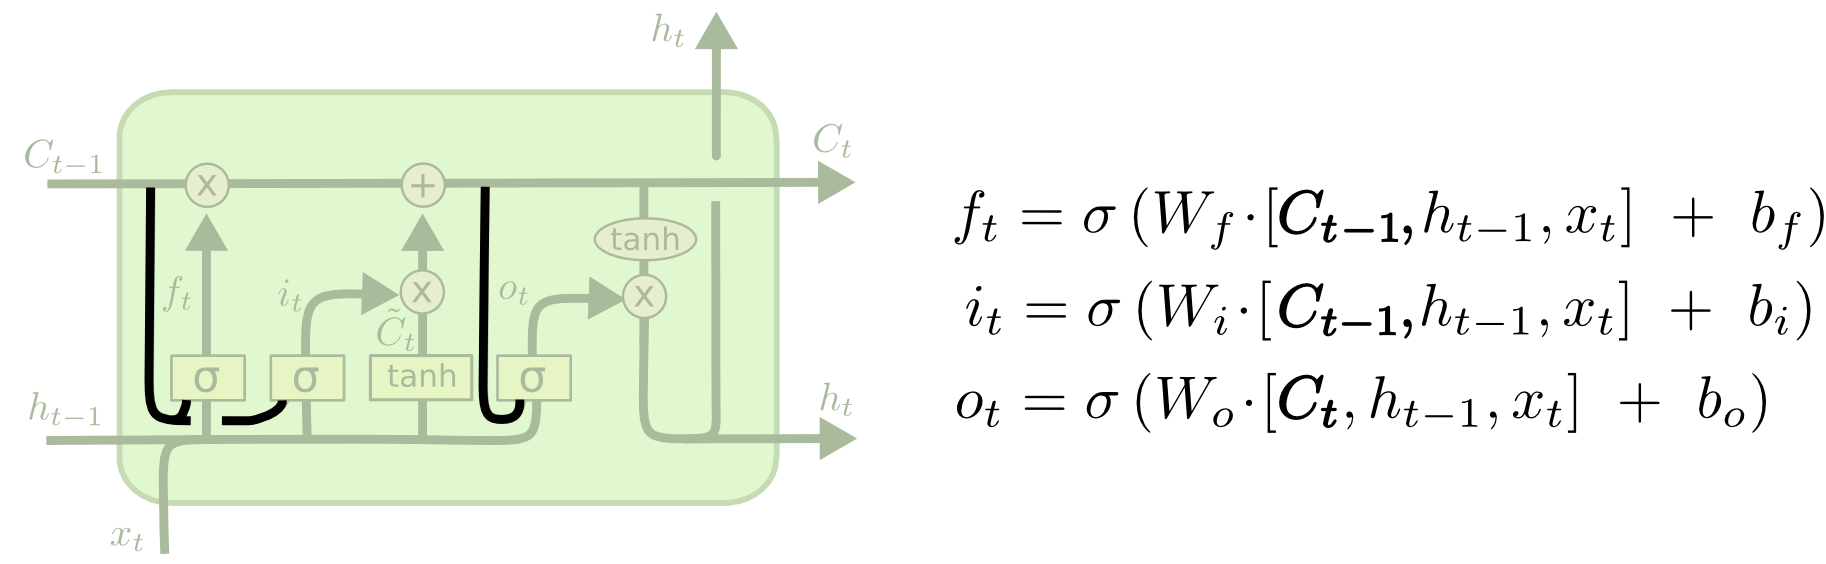
\includegraphics[width=0.8\linewidth]{../Report/imgs/lstm_peepholes}}
	\end{figure}
	
	Все фильтры <<подглядывают>> вектор состояния $C_{t-1}$ или $C_t$.
	
	\medskip
	
	Увеличивается число параметров модели.
	
	\medskip
	
	Замочную скважину можно использовать не для всех фильтров.\\
	
	\textbf{LSTM Gated recurrent units (GRU)}
	
	\begin{figure}[h]
		\center{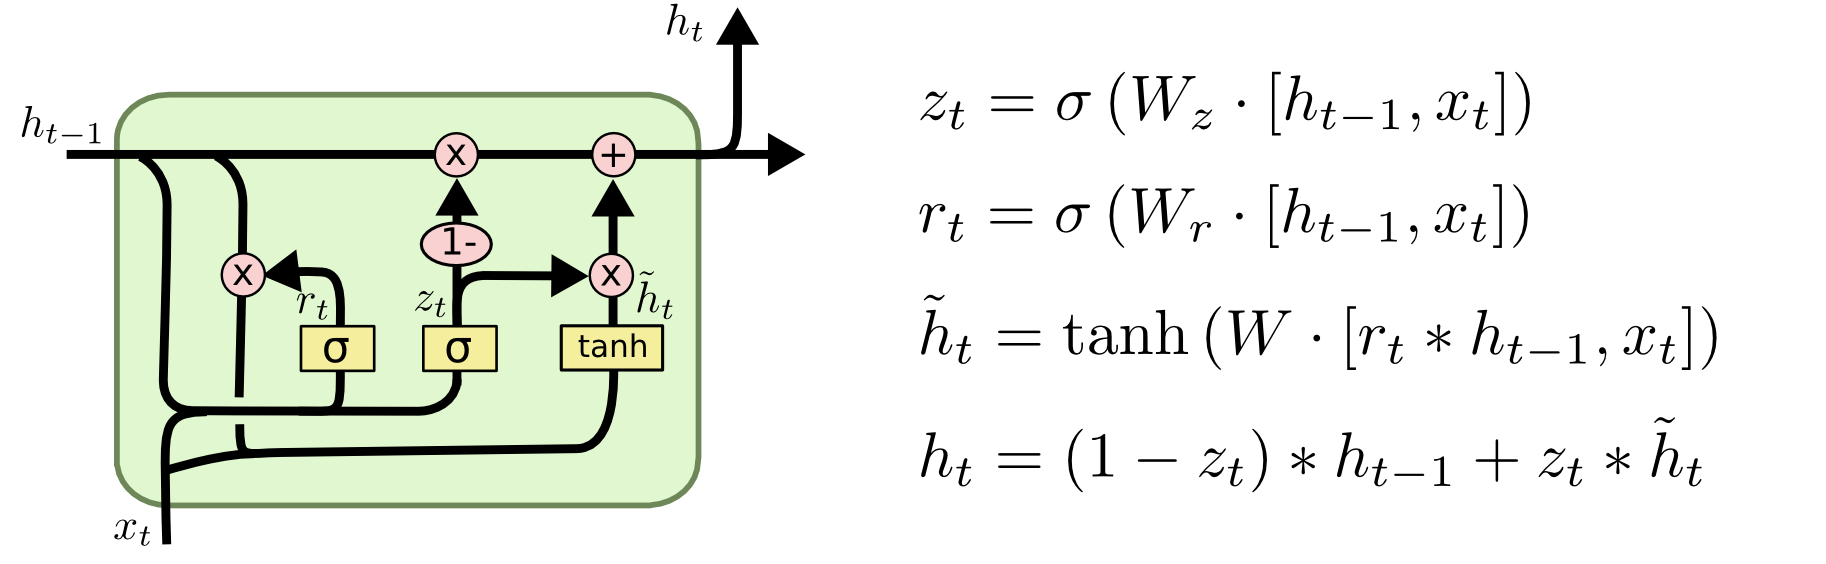
\includegraphics[width=0.8\linewidth]{../Report/imgs/lstm_gru}}
	\end{figure}
	
	Используется только состояние $h_t$, вектор $C_t$ не вводится.
	
	\medskip
	
	Фильтр обновления (update gate) вместо входного и забывающего.
	
	\medskip
	
	Фильтр перезагрузки (reset gate) решает, какую часть памяти нужно перенести дальше с прошлого шага.
	
	
	
	\section{Dropout}
	
	Главная идея Dropout — вместо обучения одной DNN обучить ансамбль нескольких DNN, а затем усреднить полученные результаты.
	\begin{figure}[h]
		\center{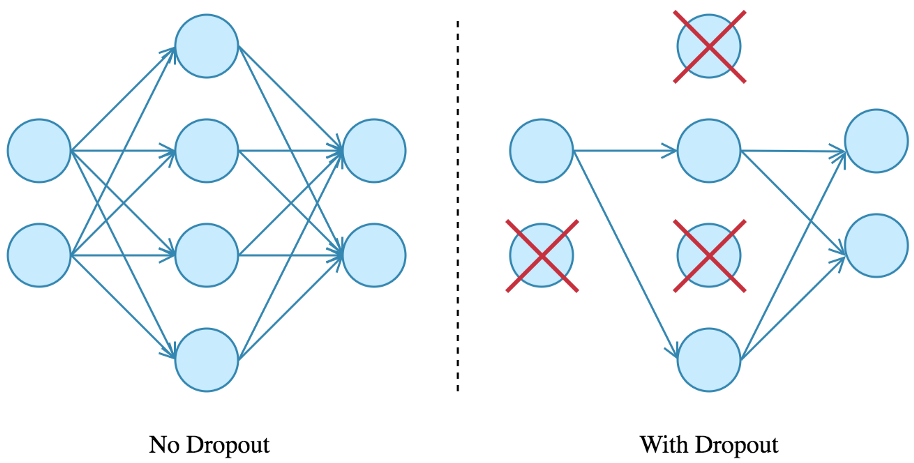
\includegraphics[width=1\linewidth]{../Report/imgs/dropout}}
	\end{figure}
	В стандартной нейронной сети производная, полученная каждым параметром, сообщает ему, как он должен измениться, чтобы, учитывая деятельность остальных блоков, минимизировать функцию конечных потерь. Поэтому блоки могут меняться, исправляя при этом ошибки других блоков. Это может привести к чрезмерной совместной адаптации (co-adaptation), что, в свою очередь, приводит к переобучению, поскольку эти совместные адаптации невозможно обобщить на данные, не участвовавшие в обучении. Мы выдвигаем гипотезу, что Dropout предотвращает совместную адаптацию для каждого скрытого блока, делая присутствие других скрытых блоков ненадежным. Поэтому скрытый блок не может полагаться на другие блоки в исправлении собственных ошибок.
	
	Обучение: обнуляем выход $h$-ого нейрона $\ell$-го слоя с вероятностью $p_\ell$.
	
	$$a^{\ell+1}_{ih} = \xi^{\ell}_h f_h^{\ell}\big( \sum\limits_{j} w_{jh}a_{ij}^{\ell} \big), P(\xi^{\ell}_h = 0) = p_\ell$$
	
	Инференс: вводим поправку
	
	$$a^{\ell+1}_{ih} = (1 - p_{\ell}) f_h^{\ell}\big( \sum\limits_{j} w_{jh}a_{ij}^{\ell} \big)$$
	
	
	Inverted Dropout: $$a^{\ell+1}_{ih} = \dfrac{1}{(1 - p_{\ell})} \xi^{\ell}_h f_h^{\ell}\big( \sum\limits_{j} w_{jh}a_{ij}^{\ell} \big)$$
	
	\begin{itemize}
		\item регуляризация: из всех сетей выбираем  более устойчивую к утрате $pN$ нейронов.
		\item сокращаем переобучение, заставляя разные части сети решать одну и ту же исходную задачу. 
	\end{itemize}
	
	
	\section{Batch Normalization}
	Обычно нейронные сети обучают пакетами - подмножество обучающего набора. $B = {x_i}$ --- пакеты данных.
	Усреднение градиентов $\mathcal{C}(w)$ по пакету ускоряет сходимость алгоритма оптимизации. $B^{\ell} = \{u_i^{\ell}\}$ --- векторы объектов $x_i$ на выходе $\ell$-го слоя.
	
	Batch Normalization:
	\begin{enumerate}
		\item Нормировать каждую $j$-ю компоненту вектора $u_i^{\ell}$ по пакету:
		
		$$ \hat{u}_{ij}^{\ell} = \dfrac{u_{ij}^{\ell} - \mu_j}{\sqrt{\sigma^2_j + \varepsilon}}; \; \; \;
		\nu_j = \dfrac{1}{|B|} \sum\limits_{x_i \in B} u_{ij}^{\ell}; \; \; \;
		\sigma^2_j = \dfrac{1}{|B|} \sum\limits_{x_i \in B} (u_{ij}^{\ell} - \nu_j)^2. $$
		\item Добавить линейный слой с настраиваемыми весами:
		$$ \tilde{u}_{ij}^{\ell} = \gamma_j^\ell \hat{u}_{ij}^{\ell} + \beta_j^\ell $$
		\item Параметры $\gamma_j^\ell$ и $\beta_j^\ell$ настраиваются с помощью back-propagation.
	\end{enumerate}
	
	Как было отмечено ранее, нормализация по пакету ускоряет сходимость алгоритма оптимизации, а также устраняет так называемую проблему внутреннего ковариантного сдвига, что тоже способствует ускорению обучения. Внутренний ковариантный сдвиг - ситуация, при которой распределение выходов скрытого слоя изменяется на каждой итерации обучения, из-за чего следующему слою придется заново подстраивать свои веса под новое распределение, что существенно тормозит процесс обучения.
	
\end{document}